% ===========================================================================
%  evnx 0.5.0 — Architecture & Contributor Guide
%  Build:  pdflatex -interaction=nonstopmode main.tex   (twice for TOC)
% ===========================================================================
\documentclass[aspectratio=169,10pt]{beamer}

\newcommand{\capturedir}{../captures}
% ---------------------------------------------------------------------------
%  evnx presentation preamble — shared by all three decks
%
%  Engine: pdfLaTeX (also builds under XeLaTeX / LuaLaTeX).
%  Packages: beamer, listings, xcolor, amssymb, newunicodechar, booktabs,
%            fancyvrb, hyperref — all in texlive-latex-recommended + beamer.
%
%  \capturedir must be defined by the including document BEFORE \input of
%  this file, e.g.  \newcommand{\capturedir}{../captures}
% ---------------------------------------------------------------------------

\usetheme{Madrid}
\usecolortheme{seahorse}
\usefonttheme{professionalfonts}
\setbeamertemplate{navigation symbols}{}
\setbeamertemplate{caption}[numbered]
\setbeamerfont{frametitle}{size=\large}
\setbeamerfont{title}{size=\LARGE,series=\bfseries}

\usepackage[T1]{fontenc}
\usepackage[utf8]{inputenc}
\usepackage{lmodern}
\usepackage{amssymb}
\usepackage{booktabs}
\usepackage{xcolor}
\usepackage{listings}
\usepackage{fancyvrb}
\usepackage{newunicodechar}
\usepackage{tikz}
\usetikzlibrary{arrows.meta,positioning,shapes.geometric,fit,backgrounds}

% ---- palette ---------------------------------------------------------------
\definecolor{evnxInk}{HTML}{1F2933}
\definecolor{evnxAccent}{HTML}{2F6F4E}
\definecolor{evnxWarn}{HTML}{B7791F}
\definecolor{evnxErr}{HTML}{B03A2E}
\definecolor{evnxOk}{HTML}{2F6F4E}
\definecolor{evnxMuted}{HTML}{6B7280}
\definecolor{evnxTermBg}{HTML}{F5F5F2}
\definecolor{evnxRule}{HTML}{D1D5DB}

\setbeamercolor{structure}{fg=evnxAccent}
\setbeamercolor{alerted text}{fg=evnxErr}

% ---- glyph mapping for body text ------------------------------------------
% evnx emits exactly these 11 non-ASCII characters (enumerated from the
% captured logs, not guessed).
\newcommand{\evnxCheck}{\textcolor{evnxOk}{\ensuremath{\checkmark}}}
\newcommand{\evnxCross}{\textcolor{evnxErr}{\ensuremath{\times}}}
\newcommand{\evnxWarnSign}{\textcolor{evnxWarn}{\textbf{!}}}

\newunicodechar{✓}{\evnxCheck}
\newunicodechar{✗}{\evnxCross}
\newunicodechar{⚠}{\evnxWarnSign}
\newunicodechar{→}{\ensuremath{\rightarrow}}
\newunicodechar{↔}{\ensuremath{\leftrightarrow}}
\newunicodechar{─}{\textendash}
\newunicodechar{—}{---}
\newunicodechar{·}{\textperiodcentered}
\newunicodechar{…}{\ldots}
\newunicodechar{•}{\textbullet}
\newunicodechar{️}{}                % U+FE0F variation selector — invisible

% ---- terminal listing style ------------------------------------------------
% `literate` is required: newunicodechar does not apply inside listings.
\lstdefinestyle{evnxterm}{
  basicstyle=\ttfamily\scriptsize,
  backgroundcolor=\color{evnxTermBg},
  frame=single,
  rulecolor=\color{evnxRule},
  framesep=4pt,
  breaklines=true,
  breakatwhitespace=false,
  columns=fullflexible,
  keepspaces=true,
  showstringspaces=false,
  upquote=true,
  extendedchars=true,
  literate=
    {✓}{{\textcolor{evnxOk}{$\checkmark$}}}1
    {✗}{{\textcolor{evnxErr}{$\times$}}}1
    {⚠}{{\textcolor{evnxWarn}{\textbf{!}}}}1
    {→}{{$\rightarrow$}}1
    {↔}{{$\leftrightarrow$}}1
    {─}{{-}}1
    {—}{{---}}1
    {·}{{$\cdot$}}1
    {…}{{\ldots}}1
    {•}{{\textbullet}}1
    {️}{{}}0
    {é}{{\'e}}1
}

\lstdefinestyle{evnxcode}{
  style=evnxterm,
  basicstyle=\ttfamily\scriptsize,
  backgroundcolor=\color{white},
}

\lstset{style=evnxterm}

% ---- helper macros ---------------------------------------------------------
% \capture{file}        — include a real captured run verbatim
% \capturepart{f}{a}{b} — include lines a..b of a captured run
\newcommand{\capture}[1]{\lstinputlisting[style=evnxterm]{\capturedir/#1}}
\newcommand{\capturepart}[3]{%
  \lstinputlisting[style=evnxterm,firstline=#2,lastline=#3]{\capturedir/#1}}

% a labelled "real output" box
\newcommand{\realrun}[1]{%
  \begin{center}\scriptsize\textcolor{evnxMuted}{real run \textendash\ #1}\end{center}}

\newcommand{\cmd}[1]{\texttt{\textbf{#1}}}
\newcommand{\flag}[1]{\texttt{#1}}
\newcommand{\file}[1]{\texttt{#1}}

% exit-code chips
\newcommand{\exitzero}{\textcolor{evnxOk}{\texttt{0}}}
\newcommand{\exitone}{\textcolor{evnxWarn}{\texttt{1}}}
\newcommand{\exittwo}{\textcolor{evnxErr}{\texttt{2}}}

% a standard "verified against" footline for factual slides
\newcommand{\verifiedon}{\tiny\textcolor{evnxMuted}{verified against evnx 0.5.0 @ 9cfe75b}}

\usepackage[colorlinks=true,linkcolor=evnxAccent,urlcolor=evnxAccent]{hyperref}


\title{Inside evnx}
\subtitle{The CLI, the ecosystem, and how to contribute}
\date{}

\begin{document}

\begin{frame}[plain]
  \titlepage
  \begin{center}\footnotesize
  \textcolor{evnxMuted}{evnx 0.5.0 @ \texttt{9cfe75b} --- every number measured,
  not estimated.}
  \end{center}
\end{frame}

\begin{frame}{Who this is for}
  Rust developers who want to contribute --- or who want to know what they are
  installing before they trust it with secrets.

  \vspace{0.8em}
  \begin{block}{What we will cover}
    \begin{enumerate}
      \item The ecosystem: four repositories and how they fit
      \item The CLI's internal structure, module by module
      \item How a command is wired, end to end
      \item The invariants: exit codes, streams, determinism
      \item The crypto boundary
      \item Testing: 987 tests and what each layer is for
      \item Contributing: build, test, conventions
    \end{enumerate}
  \end{block}
\end{frame}

\begin{frame}{Contents}\tableofcontents[hideallsubsections]\end{frame}

% =========================================================================
\section{The ecosystem}

\begin{frame}{Four repositories, one product}
  \begin{center}
  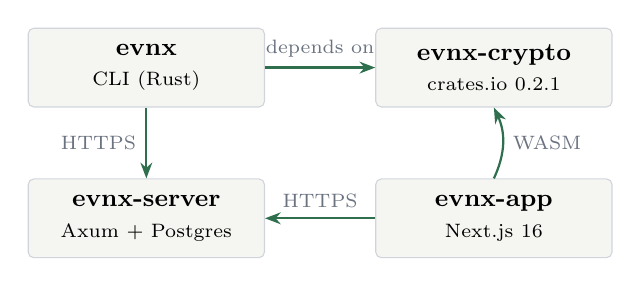
\begin{tikzpicture}[
    node distance=0.9cm and 1.4cm,
    box/.style={draw=evnxRule, fill=evnxTermBg, rounded corners=2pt,
                minimum width=3.0cm, minimum height=1.0cm, align=center,
                font=\small},
    lbl/.style={font=\scriptsize, text=evnxMuted},
    arr/.style={-{Stealth[length=2mm]}, draw=evnxAccent, thick}]

    \node[box] (cli)    {\textbf{evnx}\\{\scriptsize CLI (Rust)}};
    \node[box, right=of cli] (crypto) {\textbf{evnx-crypto}\\{\scriptsize crates.io 0.2.1}};
    \node[box, below=of cli] (server) {\textbf{evnx-server}\\{\scriptsize Axum + Postgres}};
    \node[box, right=of server] (app)  {\textbf{evnx-app}\\{\scriptsize Next.js 16}};

    \draw[arr] (cli) -- node[lbl, above]{depends on} (crypto);
    \draw[arr] (cli) -- node[lbl, left]{HTTPS} (server);
    \draw[arr] (app) -- node[lbl, above]{HTTPS} (server);
    \draw[arr] (app.north) to[bend right=25] node[lbl, right]{WASM} (crypto.south);
  \end{tikzpicture}
  \end{center}

  \vspace{0.4em}
  \begin{tabular}{@{}lll@{}}
    \toprule
    \textbf{Repo} & \textbf{Role} & \textbf{Endpoint} \\
    \midrule
    \texttt{evnx}        & The CLI binary & --- \\
    \texttt{evnx-crypto} & All key handling, shared & crates.io + npm (WASM) \\
    \texttt{evnx-server} & Stores ciphertext only & \texttt{api.evnx.dev} \\
    \texttt{evnx-app}    & Browser client & \texttt{app.evnx.dev} \\
    \bottomrule
  \end{tabular}
\end{frame}

\begin{frame}{Why the crypto is a separate crate}
  \begin{block}{One audited implementation, two consumers}
    The CLI links it as a Rust crate. The browser app loads the \emph{same code}
    compiled to WebAssembly. A bug fixed once is fixed in both, and there is no
    second implementation to drift.
  \end{block}

  \vspace{0.6em}
  \begin{alertblock}{Never a path dependency}
    \texttt{evnx-crypto = \{ version = "0.2.1" \}} --- from the registry, with a
    checksum in \file{Cargo.lock}. Cargo always prefers a \texttt{path} over the
    registry and never falls back, so a manifest carrying one fails in any
    checkout without the sibling directory. Local iteration goes in
    \file{.cargo/config.toml} via \texttt{[patch.crates-io]} instead.
  \end{alertblock}

  \vspace{0.4em}
  {\footnotesize The server uses the crate too --- but only in tests, and only
  for SRP.}
\end{frame}

\begin{frame}{What the server can and cannot see}
  \begin{center}
  \begin{tabular}{@{}ll@{}}
    \toprule
    \textbf{The server stores} & \textbf{The server never sees} \\
    \midrule
    Opaque ciphertext blobs & Your master password \\
    An SRP \emph{verifier} & Your vault keys \\
    Wrapped vault keys (it cannot unwrap) & Any plaintext value \\
    BLAKE3 hashes of tokens and IPs & A raw IP address \\
    Variable \emph{names} and versions & Variable \emph{values} \\
    \bottomrule
  \end{tabular}
  \end{center}

  \vspace{0.8em}
  \begin{block}{Enforced, not promised}
    Migration 006 makes the audit log append-only with database triggers ---
    the database refuses what the application merely never did. Migration 004
    adds a CHECK constraint that makes half a key-wrap unstorable.
  \end{block}
\end{frame}

% =========================================================================
\section{Inside the CLI}

\begin{frame}[fragile]{The shape of the crate}
  \capturepart{70-codebase-layout.txt}{1}{14}

  \begin{columns}[T]
    \begin{column}{0.5\textwidth}
      {\footnotesize
      \texttt{cli.rs} --- the whole clap surface\\
      \texttt{main.rs} --- dispatch + exit codes\\
      \texttt{lib.rs} --- the library face\\
      \texttt{commands/} --- one module per command}
    \end{column}
    \begin{column}{0.5\textwidth}
      {\footnotesize
      \texttt{core/} --- parser, config, spec, gitignore\\
      \texttt{cloud/} --- everything behind \texttt{--features cloud}\\
      \texttt{schema/} --- the component catalogue\\
      \texttt{utils/} --- terminal UI, strings, fs}
    \end{column}
  \end{columns}
\end{frame}

\begin{frame}[fragile]{By the numbers}
  \capturepart{70-codebase-layout.txt}{15}{45}
\end{frame}

\begin{frame}[fragile]{A command is four files, not one}
  \capturepart{91-module-detail.txt}{1}{9}

  \begin{block}{The split is deliberate}
    \texttt{detector} decides \emph{what} is a secret. \texttt{runner}
    orchestrates. \texttt{models} is the data. \texttt{output} renders --- and
    it renders four formats from one model, which is why \texttt{pretty},
    \texttt{json}, \texttt{sarif} and \texttt{github} cannot disagree about what
    was found.
  \end{block}
\end{frame}

\begin{frame}{Feature flags: what compiles when}
  \begin{center}
  \begin{tabular}{@{}lll@{}}
    \toprule
    \textbf{Feature} & \textbf{Pulls in} & \textbf{Gives you} \\
    \midrule
    (default)   & --- & init, validate, scan, diff, convert, sync, template, doctor, spec \\
    \texttt{migrate} & \texttt{reqwest}, \texttt{crypto\_box} & \cmd{evnx migrate} \\
    \texttt{backup}  & \texttt{aes-gcm}, \texttt{argon2}, \texttt{rand} & \cmd{backup}, \cmd{restore} \\
    \texttt{cloud}   & \texttt{evnx-crypto}, \texttt{reqwest}, \texttt{blake3}, \texttt{qrcode} & \cmd{auth}, \cmd{vault}, \cmd{cloud} \\
    \texttt{full}    & \texttt{migrate} + \texttt{backup} & --- \\
    \bottomrule
  \end{tabular}
  \end{center}

  \vspace{0.7em}
  \begin{alertblock}{\texttt{cloud} is deliberately not in \texttt{full}}
    Adding it would silently change what \texttt{full} means for people already
    using that flag. But the \textbf{prebuilt binaries do ship it} ---
    \texttt{release.yml} builds with \flag{--all-features}, and membership in
    \texttt{full} is irrelevant to that. Only \texttt{cargo install} compiles
    with \texttt{default = []}.
  \end{alertblock}
\end{frame}

% =========================================================================
\section{How a command is wired}

\begin{frame}[fragile]{1. Declare it in \file{cli.rs}}
  \capturepart{90-wiring.txt}{3}{16}

  {\footnotesize The doc comment \emph{is} the help text. \texttt{after\_help}
  comes from \file{docs.rs} --- clap collapses a fenced block in a doc comment
  into one unusable line, so examples live in \texttt{after\_help} where they
  pass through verbatim.}
\end{frame}

\begin{frame}[fragile]{2. Dispatch in \file{main.rs}, 3. Implement in \file{commands/}}
\begin{lstlisting}[style=evnxcode,language=Rust]
// main.rs
Commands::Scan { path, exclude, pattern, severity, format, exit_zero, .. } => {
    // config < flag precedence, resolved here
    let severity = core::config::pick(severity, cfg.scan.severity);
    commands::scan::run(...)   // returns Result<()>
}
\end{lstlisting}

  \vspace{0.4em}
\begin{lstlisting}[style=evnxcode,language=Rust]
// commands/scan/mod.rs
pub fn run(opts: ScanOptions) -> Result<()> {
    let files   = filters::collect(&opts)?;      // what to read
    let results = runner::scan(files, &opts)?;   // what was found
    output::render(&results, opts.format)?;      // how to say it
    std::process::exit(results.exit_code());     // 0 / 1 / 2
}
\end{lstlisting}

  {\footnotesize Illustrative shape, not a literal paste --- the real signatures
  carry more context.}
\end{frame}

\begin{frame}[fragile]{4. The exit code is decided in one place}
  \capturepart{76-main-exit-tail.txt}{5}{29}
\end{frame}

% =========================================================================
\section{The invariants}

\begin{frame}{Four rules the codebase holds itself to}
  \begin{enumerate}
    \item \textbf{\exittwo{} means no verdict.} An error is never \exitone.
          Decided centrally in \texttt{main}, so a command added later inherits
          it rather than remembering.
    \item \textbf{Machine output on stdout, humans on stderr.} Every format.
          \texttt{evnx scan --format sarif > f.sarif} is always clean.
    \item \textbf{Deterministic output.} Findings come out in file order, every
          run. A hash-ordered collection leaking into output is a bug --- it was
          one, and it is now pinned by a golden test with five findings.
    \item \textbf{Values are masked everywhere.} First-4/last-4, in all four
          formats. A scanner that prints secrets into a CI log has not helped.
  \end{enumerate}

  \vspace{0.6em}
  \begin{block}{Why these are load-bearing}
    Each one is the difference between a tool you can put in a pipeline and a
    tool you have to babysit.
  \end{block}
\end{frame}

\begin{frame}{The parser is stricter than you expect --- on purpose}
  \begin{center}
  \begin{tabular}{@{}ll@{}}
    \toprule
    \textbf{Accepted} & \textbf{Rejected} \\
    \midrule
    \texttt{FOO=bar} & \texttt{1DIGIT=x} (leading digit) \\
    \texttt{export FOO=bar} & \texttt{HAS-DASH=x} \\
    \texttt{\_LEADING=1} & \texttt{SPACED KEY=x} \\
    \texttt{\_\_DOUBLE=1} & \texttt{=noKey} \\
    quoted, multi-line values & \texttt{NO\_EQUALS} \\
    \bottomrule
  \end{tabular}
  \end{center}

  \vspace{0.7em}
  \begin{alertblock}{One parser, one answer}
    \cmd{doctor} used to carry its own line-syntax regex and disagreed with the
    core parser in \emph{both} directions --- rejecting valid \texttt{export},
    accepting a leading underscore the parser refused. A test now runs both over
    one corpus and requires the same verdict.
  \end{alertblock}
\end{frame}

% =========================================================================
\section{The crypto boundary}

\begin{frame}[fragile]{What \texttt{evnx-crypto} exposes}
  \capturepart{78-crypto-server.txt}{2}{30}
\end{frame}

\begin{frame}{Three rules the API enforces}
  \begin{enumerate}
    \item \textbf{Key bytes are private.} \texttt{MasterKey}, \texttt{VaultKey}
          and \texttt{SecretArray} expose bytes only through \texttt{.expose()},
          and cannot be built from arbitrary bytes outside the crate.
    \item \textbf{Everything zeroizes on drop.} \texttt{ZeroizeOnDrop} on every
          struct that touches key material.
    \item \textbf{Blobs carry associated data.} \texttt{encrypt\_vault} and
          \texttt{decrypt\_vault} take an \texttt{aad} that must match, and it is
          \texttt{vault\_aad(vault\_id, version)}.
  \end{enumerate}

  \vspace{0.6em}
  \begin{block}{What the AAD buys}
    A malicious server cannot replay an old version as current. The consequence
    for callers: a \texttt{409} conflict requires \textbf{re-encryption}, not a
    bare retry --- the version number is authenticated into the ciphertext.
  \end{block}

  \vspace{0.3em}
  {\footnotesize Passing \texttt{b""} disables that protection. Do not.}
\end{frame}

\begin{frame}[fragile]{Randomness: one lesson worth carrying}
  \begin{alertblock}{What was shipped}
\begin{semiverbatim}\scriptsize
let seed = SystemTime::now().duration_since(UNIX_EPOCH)
             .unwrap().as_nanos();
format!("\{:064x\}", seed ^ 0x5DEECE66D)
\end{semiverbatim}
  With the comment: \emph{``Simple time-based entropy for demo; replace with
  crypto RNG in production.''} It was not replaced.
  \end{alertblock}

  \vspace{0.5em}
  A \texttt{u128} of nanoseconds occupies about 61 bits, so 48 of the 64 hex
  characters were always \texttt{0}. Roughly 25 bits --- of \emph{time}, not
  randomness --- and evnx printed \emph{``Generated secure secret''} over it.

  \vspace{0.6em}
  \begin{block}{The test that let it through}
    \texttt{assert\_eq!(secret.len(), 64)}. It checked the \textbf{shape} and
    never the \textbf{property}. The replacement asserts distinctness, absence
    of a shared prefix, and that the value is not mostly zeros.
  \end{block}

  {\footnotesize Now 32 bytes from the OS CSPRNG via \texttt{getrandom}, which
  panics rather than falling back --- a silent downgrade to a weaker source is
  exactly the bug being replaced.}
\end{frame}

% =========================================================================
\section{Testing}

\begin{frame}[fragile]{987 tests, in layers}
  \capturepart{72-test-run.txt}{1}{18}
\end{frame}

\begin{frame}{What each layer is for}
  \begin{tabular}{@{}p{0.28\textwidth}p{0.66\textwidth}@{}}
    \toprule
    \textbf{Layer} & \textbf{Guards} \\
    \midrule
    Unit (in-module)   & Parsing, detection, formatting, key rules \\
    \texttt{tests/*\_integration.rs} & A command end to end, in a temp directory \\
    \texttt{tests/golden\_output.rs} & Byte-exact machine output \\
    \texttt{tests/devrel\_review.rs} & One test per reported finding, keyed by id \\
    Doc tests          & Every example in a doc comment actually compiles \\
    \bottomrule
  \end{tabular}

  \vspace{0.7em}
  \begin{block}{Golden files are a contract with other programs}
    \texttt{scan --format json|sarif|github}, \texttt{validate --format json},
    \texttt{diff --format json}, \texttt{convert} --- all pinned. A change to any
    of them is now a deliberate act, and the failure message tells you to
    re-generate with \texttt{UPDATE\_GOLDEN=1} if you meant it.
  \end{block}
\end{frame}

\begin{frame}{Two testing lessons from this codebase}
  \begin{alertblock}{A fixture with one item cannot catch an ordering bug}
    The golden files pinned machine output --- but every fixture had at most
    \textbf{one} finding, and one item is never out of order. Output was
    non-deterministic for months underneath a passing suite. The fixture now has
    five.
  \end{alertblock}

  \vspace{0.6em}
  \begin{alertblock}{Three tests were found asserting the bug}
    \texttt{test\_validate\_url} asserted
    \texttt{!validate\_url("ftp://example.com")}.
    \texttt{force\_overwrites\_the\_example} asserted a string with no trailing
    newline. Each pinned the defect it was meant to guard against.
  \end{alertblock}

  \vspace{0.5em}
  {\footnotesize \textbf{Sabotage verification} is the house practice: revert the
  fix, re-run, and watch the \emph{specific} test fail with a message naming what
  broke. A fix whose test still passes when reverted is not tested.}
\end{frame}

% =========================================================================
\section{Contributing}

\begin{frame}[fragile]{Getting started}
\begin{lstlisting}[style=evnxcode,language=bash]
git clone https://github.com/urwithajit9/evnx && cd evnx

cargo build --release --all-features     # ~60s cold
cargo test  --all-features               # 987 tests
cargo clippy --all-features --all-targets -- -D warnings
cargo fmt --all --check

./target/release/evnx --version          # evnx 0.5.0
\end{lstlisting}

  \vspace{0.4em}
  \begin{tabular}{@{}ll@{}}
    Rust edition & 2021, MSRV \textbf{1.85} (from \texttt{evnx-crypto}) \\
    Dependencies & 30 direct, 370 in the lockfile \\
    Binary       & 8.5\,MB, statically linked for musl targets \\
  \end{tabular}
\end{frame}

\begin{frame}[fragile]{The lints must be clean}
  \capture{73-clippy.txt}

  \begin{block}{CI runs}
    \texttt{fmt} $\rightarrow$ \texttt{clippy --all-targets -D warnings}
    $\rightarrow$ \texttt{test --all-features} $\rightarrow$ \texttt{cargo audit}
    $\rightarrow$ \texttt{cargo publish --dry-run}.
  \end{block}
\end{frame}

\begin{frame}[fragile]{House conventions}
  \begin{itemize}
    \item \texttt{thiserror} in library code, \texttt{anyhow} in binaries.
    \item \textbf{No \texttt{.unwrap()} in production paths.}
    \item Key material: \texttt{ZeroizeOnDrop}, always.
    \item Never log a secret value, key material, or a raw IP.
    \item An error message names \textbf{what} failed, \textbf{where}, and
          \textbf{what to do} --- and says what was \emph{not} done.
    \item A doc comment that shows a command must show one that runs.
  \end{itemize}

  \vspace{0.7em}
  \begin{block}{The error style, by example}
\begin{semiverbatim}\scriptsize
Error: 1 variable referenced in app.yaml.tpl has no value in .env: OTEL_ENDPOINT

Define it there, or give it a fallback with \{\{NAME|default:value\}\}.
Nothing was written to app.yaml.
\end{semiverbatim}
  \end{block}
\end{frame}

\begin{frame}{Where to start}
  \begin{tabular}{@{}p{0.30\textwidth}p{0.64\textwidth}@{}}
    \toprule
    \textbf{Interest} & \textbf{Look at} \\
    \midrule
    Detection rules & \file{src/commands/scan/detector.rs} --- add a provider format \\
    Output formats  & \file{src/commands/scan/output.rs} + a golden fixture \\
    New components  & \file{src/schema/} --- the \flag{--with} catalogue \\
    Parsing         & \file{src/core/parser.rs} --- 1{,}111 lines, heavily tested \\
    Cloud           & \file{src/cloud/} --- needs \texttt{--features cloud} \\
    Cryptography    & the \texttt{evnx-crypto} repository, not this one \\
    \bottomrule
  \end{tabular}

  \vspace{0.8em}
  \begin{block}{Good first contributions}
    A new provider key format (detector + fixture + test), a new
    \cmd{convert} target, a component for \flag{--with}, or a doc comment for
    a flag whose help is thin.
  \end{block}
\end{frame}

\begin{frame}{The one rule that matters most}
  \begin{center}
  \vspace{0.5em}
  {\Large Every file evnx \textbf{generates} or \textbf{repairs}\\[0.3em]
  must pass every other evnx command.}
  \end{center}

  \vspace{1em}
  This single invariant would have caught, before release:
  \begin{itemize}\footnotesize
    \item \cmd{init} writing a \texttt{DATABASE\_URL} that
          \cmd{validate --validate-formats} rejected
    \item \cmd{init} writing a \file{.env} whose every line was commented out,
          so \cmd{validate} reported all of it missing
    \item \cmd{init} writing a \file{.env.example} with no trailing newline, so
          the next appended variable silently vanished
    \item \cmd{validate --fix} generating a secret that \cmd{scan} then called weak
  \end{itemize}

  \vspace{0.8em}
  \begin{center}
  \url{https://github.com/urwithajit9/evnx}
  \end{center}
\end{frame}

\end{document}
